%-------------------------------------------------------------------------
% info-S1-controles.tex
%-------------------------------------------------------------------------
\marginpar{\footnotesize\bf
{\large\bf Sommaire}\\[2mm]
\mbox{}\hfill
\begin{minipage}{7.75cm}
{CAF1 : calculs booléens}\ \dotfill\ \pageref{caf1}\\
{CAF2 : codage des nombres}\ \dotfill\ \pageref{caf2}\\
{CAF3 : recherche d'un élément}\ \dotfill\ \pageref{caf3}\\
{DS1 : instructions de base}\ \dotfill\ \pageref{ds1}\\
{DS2 : procédures et fonctions}\ \dotfill\ \pageref{ds2}\\
\mbox{}
\end{minipage}
}
Cette annexe propose des exemples corrigés de contrôles d'autoformation (CAF)
et de contrôles de compétences (DS) tels qu'ils sont programmés
au cours du semestre S1 (voir le planning prévisionnel en section \ref{annexe:planning} page \pageref{annexe:planning}).
L'esprit de ces contrôles est résumé dans le chapitre \ref{ch:introduction} d'introduction à la section
\ref{sub:evaluation} page \pageref{sub:evaluation}.

Quel que soit le type de contrôle, un exercice cherche à évaluer un objectif
particulier. Aussi, la notation exprimera la distance qui reste à parcourir 
pour atteindre cet objectif (figure \ref{fig:cibleAnnexe}): 
\marginpar{\footnotesize\em
\fbox{\begin{minipage}{8cm}\label{fig:cibleAnnexe}
Notation : la métaphore de la cible.
$$\includegraphics{cible.pdf}$$
\end{minipage}}

\begin{rem} Une absence à un contrôle conduit à la note 4 
(« la cible n'est pas visée »). 
\end{rem}
}
$$\begin{tabular}{l@{ : }l@{ $\rightarrow$ }l}
0 & «~en plein dans le mille !~» & l'objectif est atteint \\
1 & «~pas mal !~» & on se rapproche de l'objectif \\
2 & «~juste au bord de la cible !~» & on est encore loin de l'objectif\\
3 & «~la cible n'est pas touchée !~» & l'objectif n'est pas atteint
\end{tabular}$$
Ainsi, et pour changer de point de vue sur la notation, le contrôle 
est réussi lorsqu'on a 0 ! Il n'y a pas non plus de $1/2$ point ou de $1/4$ 
de point : le seul barême possible ne comporte que 4 niveaux : 0, 1, 2 et 3.
On ne cherche donc pas à «~grappiller~» des points : 
\begin{itemize}
\item on peut avoir 0 (objectif atteint) et avoir fait une ou deux erreurs 
	bénignes en regard de l'objectif recherché;
\item on peut avoir 3 (objectif non atteint) et avoir quelques éléments de
	réponse corrects mais sans grand rapport avec l'objectif.
\end{itemize}

%-------------------------------------------------------------------------
\newpage
\section*{CAF1 : calculs booléens}\label{caf1}
%-------------------------------------------------------------------------
\index{evaluation@évaluation!contrôle d'autoformation}
\index[td]{contrôle d'autoformation}

%-----------------------------------------------------------------------------
\subsection*{Développement d'une expression booléenne}
Développer l'expression booléenne suivante : 
$$t = \overline{a \cdot b \cdot c \cdot d}$$
$$\framebox[13.5cm]{\color{red}
$\begin{array}{llll}
t &=& \overline{a \cdot b \cdot c \cdot d} & \\
  &=& \overline{(a \cdot b) \cdot (c \cdot d)} & \mbox{associativité}\\ 
  &=& \overline{a \cdot b} + \overline{c \cdot d} & \mbox{De Morgan}\\ 
  &=& (\overline{a} + \overline{b}) + (\overline{c} + \overline{d}) & \mbox{De Morgan}\\
  &=& \overline{a} + \overline{b} + \overline{c} + \overline{d} & \mbox{associativité}
\end{array}$}$$

%-----------------------------------------------------------------------------
\subsection*{Table de vérité d'une expression booléenne}
Etablir la table de vérité de l'expression booléenne suivante :
$$t = ((a \Rightarrow b) \cdot (b \Rightarrow c)) \Rightarrow (\overline{c} \Rightarrow \overline{a})$$
$$\framebox[13.5cm]{\color{red}
\begin{minipage}{13cm}
On pose $u = (a \Rightarrow b) \cdot (b \Rightarrow c)$ :

$$\begin{array}{|ccc|ccc|ccc|c|}
\hline
a & b & c & (a \Rightarrow b) & (b \Rightarrow c) & u & \overline{c} & \overline{a} & (\overline{c} \Rightarrow \overline{a}) & t \\
\hline
0 & 0 & 0 &   1 & 1 & 1 &   1 & 1 & 1 &   1\\
0 & 0 & 1 &   1 & 1 & 1 &   0 & 1 & 1 &   1\\
0 & 1 & 0 &   1 & 0 & 0 &   1 & 1 & 1 &   1\\
0 & 1 & 1 &   1 & 1 & 1 &   0 & 1 & 1 &   1\\
1 & 0 & 0 &   0 & 1 & 0 &   1 & 0 & 0 &   1\\
1 & 0 & 1 &   0 & 1 & 0 &   0 & 0 & 1 &   1\\
1 & 1 & 0 &   1 & 0 & 0 &   1 & 0 & 0 &   1\\
1 & 1 & 1 &   1 & 1 & 1 &   0 & 0 & 1 &   1\\
\hline
\end{array}$$
\end{minipage}}$$

%-----------------------------------------------------------------------------
\subsection*{Table de vérité d'un circuit logique}
On considère les conventions graphiques traditionnelles pour les opérateurs logiques $\cdot$, $+$ et $\oplus$ :
\centerline{\begin{tabular}{ccc}
$a \cdot b$ & $a + b$ & $a \oplus b$ \\
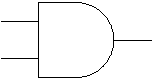
\includegraphics{et.pdf} & 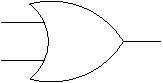
\includegraphics{ou.pdf} & \includegraphics{xor.pdf}
\end{tabular}}

Etablir la table de vérité du circuit logique ci-dessous où $a$, $b$
et $c$ sont les entrées, $x$ et $y$ les sorties.

$$\includegraphics[width=6cm]{add3.pdf}$$
$$\framebox[13.5cm]{\color{red}
\begin{minipage}{13cm}

$$\begin{array}{|ccc|ccc|cc|}
\hline
a & b & c & (b \cdot c) & (b \oplus c) & (a \cdot (b \oplus c)) & x & y \\
\hline
0 & 0 & 0 &   0 & 0 & 0 &   0 & 0 \\
0 & 0 & 1 &   0 & 1 & 0 &   1 & 0 \\
0 & 1 & 0 &   0 & 1 & 0 &   1 & 0 \\
0 & 1 & 1 &   1 & 0 & 0 &   0 & 1 \\
1 & 0 & 0 &   0 & 0 & 0 &   1 & 0 \\
1 & 0 & 1 &   0 & 1 & 1 &   0 & 1 \\
1 & 1 & 0 &   0 & 1 & 1 &   0 & 1 \\
1 & 1 & 1 &   1 & 0 & 0 &   1 & 1 \\
\hline
\end{array}$$

Il s'agit de l'addition des 3 bits $a$, $b$ et $c$ : $x$ est la somme et
$y$ la retenue

$$\begin{tabular}{r}
$a$ \\
$b$ \\
$c$ \\
\hline
$yx$
\end{tabular}
\hspace*{5mm}
\begin{tabular}{r}
0 \\
0 \\
0 \\
\hline
00
\end{tabular}
\hspace*{2mm}
\begin{tabular}{r}
0 \\
0 \\
1 \\
\hline
01
\end{tabular}
\hspace*{2mm}
\begin{tabular}{r}
0 \\
1 \\
0 \\
\hline
01
\end{tabular}
\hspace*{2mm}
\begin{tabular}{r}
0 \\
1 \\
1 \\
\hline
10
\end{tabular}
\hspace*{2mm}
\begin{tabular}{r}
1 \\
0 \\
0 \\
\hline
01
\end{tabular}
\hspace*{2mm}
\begin{tabular}{r}
1 \\
0 \\
1 \\
\hline
10
\end{tabular}
\hspace*{2mm}
\begin{tabular}{r}
1 \\
1 \\
0 \\
\hline
10
\end{tabular}
\hspace*{2mm}
\begin{tabular}{r}
1 \\
1 \\
1 \\
\hline
11
\end{tabular}$$

\end{minipage}}$$
%-----------------------------------------------------------------------------

%-------------------------------------------------------------------------
\newpage
\section*{CAF2 : codage des nombres}\label{caf2}
%-------------------------------------------------------------------------
\index{evaluation@évaluation!contrôle d'autoformation}
\index[td]{contrôle d'autoformation}

\subsection*{Représentation en complément à 2}
\begin{enumerate}
\item Déterminer la plage de valeurs entières possibles lorsqu'un
	entier positif, négatif ou nul est codé en binaire 
	sur $k = 4$ chiffres dans la représentation en complément à 2.
	
	$$\framebox[13.5cm]{\color{red}\begin{minipage}{13cm}
	Lors d'un codage en binaire sur $k$ bits, 
	seuls les nombres entiers relatifs $n$ 
	tels que $-2^{k-1} \leq n < 2^{k-1}$ peuvent être représentés 
	($\displaystyle n \in [-2^{k-1};2^{k-1}[$).
	\vspace*{3mm}
	
	Application numérique : $k=4 : [-2^{4-1};2^{4-1}[ \ = [-8;+8[$
	\end{minipage}}$$

\item Coder l'entier $n = (- 93)_{10}$ sur $k = 8$ chiffres en base $b = 2$
	en utilisant la représentation du complément à 2.
	
	$$\framebox[13.5cm]{\color{red}
\begin{minipage}{13cm}
\begin{enumerate}
\item coder $|n|=(93)_{10}$ sur $(k-1) = 7$ chiffres :
	$(93)_{10} = (1011101)_2$ 
\item mettre le bit de poids fort ($k^{\grave eme}$ bit) à $0$ :
        $(01011101)_2$ 
\item inverser tous les bits obtenus :
        $(01011101)_2 \rightarrow (10100010)_2$
\item ajouter 1 : 
	$(10100010)_2 + (00000001)_2 = (10100011)_2$
\item conclusion :
	$n = (-93)_{10} = (10100011)_2$
\end{enumerate}
\end{minipage}}$$

\item Vérifier la réponse précédente en additionnant en base $b=2$,
	$n$ et $(-n)$, codés sur $k = 8$ chiffres dans la représentation
	du complément à 2.

	$$\framebox[13.5cm]{\color{red}\begin{minipage}{13cm}
$\begin{array}{lrrrrr}
  & n &=& (- 93)_{10} &=& \ (10100011)_2\\[3mm]
+ & (-n) &=& (+ 93)_{10} &=& \ (01011101)_2\\[3mm]
\hline
\\[-2mm]
= & 0 &=& (0)_{10} &=& \ 1(00000000)_2
\end{array}$
\vspace*{3mm}

Le bit de poids fort (le $9^{\grave eme}$ bit à partir de la droite : {\tt 1})
est perdu.
\end{minipage}}$$
\end{enumerate}

%-----------------------------------------------------------------------------
\subsection*{IEEE 754 simple précision}
Coder le nombre réel $x=-73.25$ selon la norme IEEE 754 en simple précision.
	
	$$\framebox[14.5cm]{\color{red}
\begin{minipage}{14cm}
\begin{description}
\item[partie entière :] : $(73)_{10} = (1001001)_2$
\item[partie fractionnaire :] $(0.25)_{10} = (0.01)_2$
\item[mantisse normalisée :] $(1001001.01)_2 =
(1.00100101)_2 \cdot 2^6 = (1.00100101)_2 \cdot 2^{(00000110)_2}$
\item[exposant relatif à 127 :] $(01111111)_2 + (00000110)_2 = (10000101)_2$
\item[signe :] $(1)_2$
\item[norme IEEE 754 :]
\end{description}
\centerline{\includegraphics[width=13.5cm]{ieee754A.pdf}}
\end{minipage}
}$$


%-------------------------------------------------------------------------
\newpage
\section*{CAF3 : recherche d'un élément}\label{caf3}
%-------------------------------------------------------------------------
\index{evaluation@évaluation!contrôle d'autoformation}
\index[td]{contrôle d'autoformation}

%-----------------------------------------------------------------------------
\subsection*{Recherche d'une occurrence}
Définir une fonction {\tt rechercheKieme} qui recherche le rang {\tt r}
de la $\mbox{\tt k}^{\grave eme}$ occurrence d'un élément {\tt x} à partir du début 
d'une liste {\tt t}.\\
Exemple : {\tt t = [7,4,3,2,4,4]}, {\tt k = 2}, {\tt x = 4} $\rightarrow$ {\tt r
= 4}

$$\begin{minipage}{15cm}\color{red}
\begin{lstlisting}
def rechercheKieme(t,x,k):
    """
    recherche la kième occurrence de x dans le tableau t
    -> (found, index)
    (found == False and index == len(t)) or
    (found == True and 0 <= index < len(t))

    >>> rechercheKieme([],7,2)
    (False, 0)
    >>> rechercheKieme([1,2,3,2],7,2)
    (False, 4)
    >>> rechercheKieme([1,2,3,2],2,2)
    (True, 3)
    """
    assert type(t) is list
    assert type(k) is int
    found, index, occur = False, 0, 0
    while index < len(t) and not found:
        if t[index] == x:
            occur = occur + 1
            if occur == k: found = True
            else: index = index + 1
        else: index = index + 1
    return found, index
\end{lstlisting}
\end{minipage}
$$

%-----------------------------------------------------------------------------
\subsection*{Exécution d'une fonction}
On considère la fonction {\tt g} ci-dessous.
$$\begin{minipage}[t]{15cm}\footnotesize
\begin{lstlisting}
def g(t,x,k,d):
    assert type(t) is list
    assert type(k) is int and k > 0
    assert d in [0,1]

    ok, i, n = False, (1-d)*(len(t)-1), 0
    print i,n,ok #-------------------------- affichage
    while i in range(0,len(t)) and not ok:
        if t[i] == x:
            n = n + 1
            if n == k: ok = True
            else: i = i - (-1)**d
        else: i = i - (-1)**d
        print i,n,ok #---------------------- affichage
    print i,n,ok #-------------------------- affichage

    return ok,i
\end{lstlisting}
\end{minipage}$$

\begin{enumerate}
\item Qu'affiche l'appel {\tt g(t,2,3,0)} quand {\tt t = [5,2,5,3,5,2,5,2]} ?
$$\framebox[5.9cm]{
\begin{minipage}{5.75cm}\tt
>>> t = [5,2,5,3,5,2,5,2]\\
>>> g(t,2,3,0)\\\color{red}
7 0 False\\
6 1 False\\
5 1 False\\
4 2 False\\
3 2 False\\
2 2 False\\
1 2 False\\
1 3 True\\
1 3 True\\
(True, 1)
\end{minipage}}$$
\end{enumerate}

\hfill

\begin{enumerate}\setcounter{enumi}{1}
\item Compléter la spécification de la fonction {\tt g}.
	\begin{description}
	\item[Description :]\mbox{} 
	
	\framebox[13.5cm]{\begin{minipage}{13cm}\color{red}\tt 
	"""\\
	(ok,i) = g(t,x,k,d)\\
	i est le rang de la kème occurence de x en partant\\
	du début (d = 1) ou de la fin (d = 0) de la liste t,\\
	si cette occurence existe (ok = True);\\
        i = d*len(t) - (1-d) sinon (ok = False)\\
	"""
	\end{minipage}}
	
	
	\item[Jeu de tests :]\mbox{} 
	
	\framebox[13.5cm]{\begin{minipage}{13cm}\color{red}\tt 
	"""\\
	>>> g([],7,2,0)\\
	(False, -1)\\
	>>> g([],7,2,1)\\
	(False, 0)\\
	>>> g([1,2,3,2,5],2,2,0)\\
	(True, 1)\\
	>>> g([1,2,3,2,5],2,2,1)\\
	(True, 3)\\
	>>> g([1,2,3,2,5],2,3,0)\\
	(False, -1)\\
	>>> g([1,2,3,2,5],2,3,1)\\
	(False, 5)\\
	"""
	\end{minipage}}
	\end{description}
\end{enumerate}

%-------------------------------------------------------------------------
\newpage
\section*{DS1 : instructions de base}\label{ds1}
%-------------------------------------------------------------------------
\index{evaluation@évaluation!contrôle de compétence}
\index[td]{contrôle de compétence}

%-----------------------------------------------------------------------------
\subsection*{Exécution d'une séquence d'instructions}
%-----------------------------------------------------------------------------
Qu'affiche la séquence d'instructions suivante ?
\vspace*{5mm}

\hspace*{5mm}\begin{py}{5cm}
\begin{verbatim}
a = 289
x = 1
z = a
y = 0
t = x
print a,x,z,t,y
while x <= a: x = x*4

print a,x,z,t,y
t = x
while x > 1:
  x = x/4
  t = t/2 - x
  if t <= z: 
    z = z - t
    t = t + x*2
  y = t/2
  print a,x,z,t,y

print a,x,z,t,y
\end{verbatim}
\end{py}\hfill
{\color{red}\begin{tabular}[t]{|c|c|c|c|c|}
\hline
\makebox[1cm]{a} & \makebox[1cm]{x} & \makebox[1cm]{z} & \makebox[1cm]{t} & \makebox[1cm]{y} \\
\hline
289 & 1 & 289 & 1 & 0 \\
\hline
289 & 1024 & 289 & 1 & 0 \\
\hline
289 & 256 & 33 & 768 & 384 \\
289 & 64 & 33 & 320 & 160 \\
289 & 16 & 33 & 144 & 72 \\
289 & 4 & 33 & 68 & 34 \\
289 & 1 & 0 & 35 & 17 \\
\hline
289 & 1 & 0 & 35 & 17 \\
\hline
\end{tabular}}
\vspace*{5mm}


Il s'agit du calcul de la racine carrée entière $y$ d'un nombre entier $a$ :
$y = 17 = \sqrt{289} = \sqrt{a}$.

%-----------------------------------------------------------------------------
\subsection*{Calcul de $\pi$}
%-----------------------------------------------------------------------------
Dans cette section, on se propose de calculer $\pi$ selon la méthode
des rectangles.

Selon cette méthode, on calcule $\pi$ \`a partir de l'expression de la 
surface $S$ d'un cercle de rayon unité.
On approche la surface du quart de cercle par $n$ rectangles 
d'aire $A_i = y_i/n$.
	
	\begin{minipage}{9cm}
	Ecrire un algorithme qui calcule $\pi$ selon la méthode des rectangles
		à l'ordre $n$.
	\end{minipage}
	\hfill
	\begin{minipage}{4cm}
	\centerline{\includegraphics[width=4cm]{rectangle.pdf}}
	\end{minipage}

$$\framebox[14.5cm]{\begin{minipage}{14cm}\color{red}
Les points du cercle de rayon unité ont pour coordonnées
	$\displaystyle x_k = \frac{k}{n}$ et $\displaystyle y_k = \sqrt{1-\frac{k^2}{n^2}}$
	et un rectangle de base a pour surface $\displaystyle s_k = \frac{1}{n}\sqrt{1-\frac{k^2}{n^2}}$.
	La surface du 1/4 de cercle s'écrit alors comme la somme des rectangles de base :
	$\displaystyle S = \frac{\pi}{4} = \sum_{k=0}^n s_k = \frac{1}{n}\sum_{k=0}^n \sqrt{1-\frac{k^2}{n^2}}$.
\vspace*{3mm}

Ce qui donne avec l'interpréteur {\tt python} :
$$\begin{py}{12cm}
\tt
>>> from math import *\\
>>> n = 20000000\\
>>> y = 0.\\
>>> for k in range(0,n+1) :\\
...\ \ \ \ y = y + sqrt(1 - (1.*k*k)/(n*n))\\
... \\
>>> pi - 4*y/n\\
-9.9986801060936159e-08\\
\mbox{}
\end{py}$$
\end{minipage}}$$ 

%-----------------------------------------------------------------------------

%-----------------------------------------------------------------------------
\subsection*{Zéro d'une fonction}
%-----------------------------------------------------------------------------
\marginpar{\footnotesize\em
\begin{rem}
Voir TD \ref{td:zero} page \pageref{td:zero}.
\end{rem}
}
Dans cette section, on recherche le zéro d'une fonction $f$ continue sur un 
intervalle $[a,b]$ telle que $f(a).f(b) < 0$ 
(il existe donc une racine de $f$ dans $]a,b[$ que nous supposerons 
unique). 

Ecrire un algorithme qui détermine le zéro de $\cos(x)$ dans $[1,2]$
	selon la méthode des tangentes.
	
	Indications : soit $x_n$ une approximation de la racine $c$ recherchée : 
	$f(c) = f(x_n) + (c-x_n)f'(x_n)$; comme $f(c) = 0$, on a : 
	$c = x_n - f(x_n)/f'(x_n)$. Posons $x_{n+1} = x_n - f(x_n)/f'(x_n)$ : 
	on peut considérer que $x_{n+1}$ est une meilleure approximation de $c$ que 
	$x_n$. On recommence le procédé avec $x_{n+1}$  et ainsi de suite jusqu'à ce 
	que $|x_{n+1}-x_n|$ soit inférieur à un certain seuil $s$.

$$\framebox[14.5cm]{\begin{minipage}{14cm}\color{red}
$$\begin{py}{12cm}
\tt
>>> from math import *\\
>>> x1 = 1.\\
>>> x2 = 2.\\
>>> s = 1.e-9\\
>>> f = cos\\
>>> df = sin\\
>>> x = x2 - f(x2)/(-df(x2))\\
>>> while fabs(x-x2) > s:\\
...   x2 = x\\
...   x = x - f(x)/(-df(x))\\
... \\
>>> cos(x)\\
6.1230317691118863e-17\\
\mbox{}
\end{py}$$
\end{minipage}}$$ 

%-----------------------------------------------------------------------------
\subsection*{Tableau d'Ibn al-Banna}
%-----------------------------------------------------------------------------
\marginpar{\footnotesize\em
\begin{rem}
Voir TD \ref{td:ibnalbanna} page \pageref{td:ibnalbanna}.
\end{rem}
}
L'exercice suivant est inspir\'e du premier chapitre du
livre « Histoire d'algo\-ri\-thmes » \cite{chabert}.
On consid\`ere ici le texte d'Ibn al-Banna concernant la multiplication
\`a l'aide de tableaux.

\begin{quote}\footnotesize
Tu construis un quadrilat\`ere que tu subdivises verticalement et
horizontalement en autant de bandes qu'il y a de positions dans les
deux nombres multipli\'es. Tu divises diagonalement les carr\'es
obtenus, \`a l'aide de diagonale allant du coin inf\'erieur gauche au
coin sup\'erieur droit.

\marginpar{\footnotesize\em
\begin{rem}\mbox{}\\
\begin{itemize}
\item L'écriture du multiplicande s'effectue de droite à gauche (exemple : 352 s'écrira donc 253).
\item L'écriture du multiplicateur s'effectue de bas en haut (exemple : {\tiny$\begin{array}{c}3\\5\\2\end{array}$} 
	s'écrira donc {\tiny$\begin{array}{c}2\\5\\3\end{array}$}).
\end{itemize}
\end{rem}
}
Tu places le multiplicande au-dessus du quadrilat\`ere, en faisant 
correspondre chacune de ses positions \`a une colonne. 
Puis, tu places le multiplicateur \`a gauche ou \`a droite du quadrilat\`ere,
de telle sorte qu'il descende avec lui en faisant correspondre \'egalement 
chacune de ses positions \`a une ligne. Puis, tu multiplies, 
l'une apr\`es l'autre, chacune des positions du multiplicande du carr\'e 
par toutes les positions du multiplicateur, et tu poses le r\'esultat 
partiel correspondant \`a chaque position dans le carr\'e o\`u se coupent 
respectivement leur colonne et leur ligne, en pla\c{c}ant les unit\'es 
au-dessus de la diagonale et les dizaines en dessous. Puis, tu
commences \`a additionner, en partant du coin sup\'erieur gauche :
tu additionnes ce qui est entre les diagonales, sans effacer, 
en pla\c{c}ant chaque nombre dans sa position, en transf\'erant 
les dizaines de chaque somme partielle \`a la diagonale suivante et
en les ajoutant \`a ce qui y figure. 

La somme que tu obtiendras sera le r\'esultat.
\end{quote}

En utilisant la m\'ethode du tableau d'Ibn al-Banna, calculer $63247\times124$ 
($= 7842628$).

$$\framebox[14.5cm]{\begin{minipage}{14cm}
$$\includegraphics[width=7cm]{ibnalbanna.pdf}$$
\end{minipage}}$$ 

%-------------------------------------------------------------------------
\newpage
\section*{DS2 : procédures et fonctions}\label{ds2}
%-------------------------------------------------------------------------
\index{evaluation@évaluation!contrôle de compétence}
\index[td]{contrôle de compétence}

%-----------------------------------------------------------------------------
\subsection*{Calcul de $\pi$}
%-----------------------------------------------------------------------------
Définir une fonction qui calcule $\pi$ à l'ordre $n$ selon la formule :
	$$\pi = 2\cdot
	\frac{4}{3}\cdot\frac{16}{15}\cdot\frac{36}{35}\cdot\frac{64}{63}\cdots =
	      2\prod_{k=1}^n\frac{4k^2}{4k^2 - 1}$$

%$$\begin{minipage}[t]{12cm}
{\color{red}
\begin{lstlisting}
def pi(n):
    """
    y = pi(n)
    calcule pi à l'ordre n
    >>> abs(pi(1) - math.pi) < 1.
    True
    >>> abs(pi(100) - math.pi) < 1./100
    True
    >>> abs(pi(10000000) - math.pi) < 1.e-7
    True
    """
    assert type(n) is int and n > 0
    y = 2.
    for k in range(1,n+1):
        u = 4*k*k
        y = y*u/(u-1)
    return y
\end{lstlisting}
}
%\end{minipage}$$

%-----------------------------------------------------------------------------
\subsection*{Conversion décimal $\rightarrow$ base $b$}
%-----------------------------------------------------------------------------
Définir une fonction qui calcule le code $t$ en base $b$ sur $k$ chiffres
d'un entier $n$.\\
Exemples pour $n=23$ : 
\begin{tabular}[t]{ll@{\ $\rightarrow$\ }l}
{\tt b = 2}  & {\tt k = 7} & {\tt t = [0, 0, 1, 0, 1, 1, 1]}\\
{\tt b = 5}  & {\tt k = 5} & {\tt t = [0, 0, 0, 4, 3]}\\
{\tt b = 21} & {\tt k = 2} & {\tt t = [1, 2]}\\
{\tt b = 25} & {\tt k = 6} & {\tt t = [0, 0, 0, 0, 0, 23]}
\end{tabular}
\marginpar{\footnotesize\em
\begin{rem}
Voir TD \ref{td:codage} page \pageref{td:codage}.
\end{rem}
}

%$$\begin{minipage}[t]{12cm}
{\color{red}
\begin{lstlisting}
def code(n,b,k):
    """
    c = code(n,b,k)
    code n en base b sur k chiffres
    >>> code(23,2,8)
    [0, 0, 0, 1, 0, 1, 1, 1]
    >>> code(23,2,7)
    [0, 0, 1, 0, 1, 1, 1]
    >>> code(23,5,5)
    [0, 0, 0, 4, 3]
    >>> code(23,21,2)
    [1, 2]
    >>> code(23,25,6)
    [0, 0, 0, 0, 0, 23]

    """
    assert type(n) is int and n >= 0
    assert type(b) is int and b > 1
    assert type(k) is int and k > 0
    c = []
    for i in range(k): c.append(0)
    q = n
    i = k-1
    while q > 0 and i >= 0:
        r = q%b
        q = q/b
        c[i] = r
        i = i - 1
    return c
\end{lstlisting}
}
%\end{minipage}$$

%-----------------------------------------------------------------------------
\subsection*{Quinconce}
%-----------------------------------------------------------------------------
\marginpar{\footnotesize\em
\begin{rem}
Voir TD \ref{td:damier} page \pageref{td:damier}.
\end{rem}
}
Définir une procédure qui dessine $n\times m$ cercles de rayon $r$
disposés en quinconce sur $n$ rangées de $m$ cercles chacune.
On utilisera les instructions de tracé {\em à la Logo}.

Organisation en quinconque : \begin{minipage}{3.5cm}\includegraphics[height=3.5cm]{quinconce.pdf}\end{minipage}

%$$\begin{minipage}[t]{15cm}
{\color{red}
\begin{lstlisting}
def quinconce(n,m,r):
    """
    quinconce(n,m,r)
    trace n rangées de m cercles de rayon r
    disposées en quinconce
    >>> quinconce(5,10,10)
    """
    assert type(n) is int and n > 0
    assert type(m) is int and m > 0
    assert type(r) is int and r > 0
    for i in range(n) :
        x0 = r*(i%2)
        y0 = 2*i*r
        for j in range(m) :
            up()
            goto(x0+2*j*r,y0)
            down()
            circle(r)           
    return
\end{lstlisting}
}
%\end{minipage}$$


%-----------------------------------------------------------------------------
\subsection*{Coefficients de Kreweras}
%-----------------------------------------------------------------------------
On consid\`ere la fonction {\tt g} ci-dessous.
$$\begin{minipage}[t]{15cm}
\begin{lstlisting}
def g(n,m):
    assert type(n) is int
    assert type(m) is int
    assert 0 <= m and m <= n
    if n == 0 and m == 0:
        c = 1
    else:
        if m == 0: c = 0
        else:
            c = 0
            for i in range(1,m+1):
                c = c + g(n-1,n-i)
    return c
\end{lstlisting}
\end{minipage}$$
\begin{enumerate}
\item Calculer toutes les valeurs possibles
	de $g(n,m)$ pour $n \in [0,6]$.
	$$\framebox[13.5cm]{\begin{minipage}{13cm}\color{red}\tt
	>>> for n in range(7):\\
        \mbox{}\ \ \ \ \ \ \ \ print 'n =', n, '\char`:',\\
        \mbox{}\ \ \ \ \ \ \ \ for m in range(n+1):\\
        \mbox{}\ \ \ \ \ \ \ \ \ \ \ \ print kreweras(n,m),\\
        \mbox{}\ \ \ \ \ \ \ \ print\\
	\mbox{}\\
	\mbox{}\\	
	n = 0  : 1\\
	n = 1  : 0 1\\
	n = 2  : 0 1 1\\
	n = 3  : 0 1 2 2\\
	n = 4  : 0 2 4 5 5\\
	n = 5  : 0 5 10 14 16 16\\
	n = 6  : 0 16 32 46 56 61 61
	\end{minipage}}$$

\item Vérifier que {\tt 12.*g(5,5)/g(6,6)} est une bonne approximation de
	$\pi$.
	$$\framebox[13.5cm]{\begin{minipage}{13cm}\color{red}\tt
	>>> 2.*6*g(5,5)/g(6,6)\\
        3.1475409836065573\\
	>>> 2.*12*g(11,11)/g(12,12)\\
	3.1416005461074121
	\end{minipage}}$$

\end{enumerate}

%-----------------------------------------------------------------------------
\subsection*{Portée des variables}
%-----------------------------------------------------------------------------
\marginpar{\footnotesize\em
\begin{rem}
Voir TD \ref{td:portee2} page \pageref{td:portee2}.
\end{rem}
}
On considère les fonctions {\tt f}, {\tt g} et {\tt h} suivantes :
\begin{center}
\begin{py}{4cm}
\begin{verbatim}
def f(x):
    x = 2*x
    print 'f', x
    return x
\end{verbatim}
\end{py}\hspace*{1cm}
\begin{py}{4cm}
\begin{verbatim}
def g(x):
    x = 4*f(x)
    print 'g', x
    return x
\end{verbatim}
\end{py}\hspace*{1cm}
\begin{py}{4cm}
\begin{verbatim}
def h(x):
    x = 3*g(f(x))
    print 'h', x
    return x
\end{verbatim}
\end{py}
\end{center}

Qu'affichent les appels suivants ?
\vspace*{2mm}

\begin{minipage}{7cm}
\begin{enumerate}
\item 

\begin{minipage}[t]{4cm}\tt
>>> x = 2\\
>>> print x\\
{\color{red}2}\\
>>> y = f(x)\\
{\color{red}f 4}\\
>>> print x\\
{\color{red}2}\\
>>> z = g(x)\\
{\color{red}f 4\\
g 16}\\
>>> print x\\
{\color{red}2}\\
>>> t = h(x)\\
{\color{red}f 4\\
f 8\\
g 32\\
h 96}\\
>>> print x\\
{\color{red}2}
\end{minipage}
\end{enumerate}
\end{minipage}
\hfill
\begin{minipage}{7cm}
\begin{enumerate}\setcounter{enumi}{1}

\item

\begin{minipage}[t]{4cm}\tt
>>> x = 2\\
>>> print x\\
{\color{red}2}\\
>>> x = f(x)\\
{\color{red}f 4}\\
>>> print x\\
{\color{red}4}\\
>>> x = g(x)\\
{\color{red}f 8\\
g 32}\\
>>> print x\\
{\color{red}32}\\
>>> x = h(x)\\
{\color{red}f 64\\
f 128\\
g 512\\
h 1536}\\
>>> print x\\
{\color{red}1536}
\end{minipage}

\end{enumerate}
\end{minipage}

%-----------------------------------------------------------------------------
\subsection*{Exécution d'une fonction itérative}
%-----------------------------------------------------------------------------
\marginpar{\footnotesize\em
\begin{rem}
Voir TD \ref{td:binome} page \pageref{td:binome}.
\end{rem}
}
On considère la procédure {\tt f} définie ci-dessous.
$$\begin{minipage}[t]{15cm}
\begin{lstlisting}
def f(n):
    for p in range(n+1):
        num = 1
        den = 1
        for i in range(1,p+1) :
            num = num*(n-i+1)
            den = den*i
        c = num/den
        print c,  #------------ affichage
    print         #------------ affichage
    return
\end{lstlisting}
\end{minipage}$$
\begin{enumerate}
\item Qu'affiche l'instruction {\tt for n in range(7): f(n)} ?
	$$\framebox[13.5cm]{\begin{minipage}{13cm}\color{red}\tt
	>>> for n in range(7): f(n)\\
	\mbox{}\\
	1\\
	1 1\\
	1 2 1\\
	1 3 3 1\\
	1 4 6 4 1\\
	1 5 10 10 5 1\\
	1 6 15 20 15 6 1
	\end{minipage}}$$
\item Que représente {\tt c} à la fin de chaque itération sur {\tt p} ?

	$$\framebox[13.5cm]{\begin{minipage}{13cm}\color{red}
	Le $p^{i\grave eme}$ coefficient du binôme $(x+y)^n$ avec $0 \leq p \leq n$.
	\end{minipage}}$$
\end{enumerate}
